\documentclass[pdftex,10pt]{book}
\RequirePackage[hyperindex,colorlinks,plainpages=false]{hyperref}
\hypersetup{pdfauthor={Heng Li},linkcolor=blue,citecolor=blue,urlcolor=blue}

\usepackage{graphicx}
\usepackage{amsmath}
\usepackage{amssymb}
\usepackage{amsthm}
\usepackage{caption}
\renewcommand{\captionfont}{\fontsize{9pt}{10pt}\selectfont}

\addtolength{\textwidth}{2cm}\addtolength{\hoffset}{-1cm}\addtolength{\textheight}{2cm}\addtolength{\voffset}{-1cm}

\DeclareMathOperator*{\argmax}{argmax}

\makeindex

\title{Mathematical Notes on SAMtools Algorithms}
\author{Heng Li}

\begin{document}

\maketitle

\chapter{Duplicate Rate}

\section{Amplicon duplicates}

Let $N$ be the number of distinct segments (or seeds) before the
amplification and $M$ be the total number of amplicons in the
library. For seed $i$ ($i=1,\ldots,N$), let $k_i$ be the number of
amplicons in the library and $k_i$ is drawn from Poinsson distribution
${\rm Po}(\lambda)$. When $N$ is sufficiently large, we have:
\[
M=\sum_{i=1}^Nk_i=N\sum_{k=0}^{\infty}kp_k=N\lambda
\]
where $p_k=e^{-\lambda}\lambda^k/{k!}$.

At the sequencing step, we sample $m$ amplicons from the library. On the
condition that:
\begin{equation}
  m\ll M
\end{equation}
we can regard this procedure as sampling with replacement. For seed $i$,
let:
\begin{equation*}
  X_i=\left\{\begin{array}{ll}
      1 & \mbox{seed $i$ has been sampled at least once} \\
      0 & \mbox{otherwise}
    \end{array}
  \right.
\end{equation*}
and then:
\begin{equation*}
  {\rm E} X_i= \Pr\{X_i=1\}=1-\Big(1-\frac{k_i}{M}\Big)^m\simeq 1-e^{-k_i m/M}
\end{equation*}
Let:
\[Z=\sum_{i=1}^NX_i\]
be the number of seeds sampled from the
library. The fraction of duplicates $d$ is:
\begin{eqnarray*}
  d&=&1-\frac{{\rm E}(Z)}{m}\\
  &\simeq&1-\frac{N}{m}\sum_{k=0}^{\infty}\big(1-e^{-km/M}\big)p_k\\
  &=&1-\frac{N}{m}+\frac{N e^{-\lambda}}{m}\sum_k \frac{1}{k!}\big(\lambda e^{-m/M}\big)^k\\
  &\simeq& 1-\frac{N}{m}\Big[1-e^{-\lambda}\cdot e^{\lambda(1-m/M)}\Big]
\end{eqnarray*}
i.e.
\begin{equation}
  d \simeq 1 - \frac{N}{m}\Big(1-e^{-m/N}\Big)
\end{equation}
irrelevant of $\lambda$. In addition, when $m/N$ is sufficiently small:
\begin{equation}\label{equ:d2}
  d\approx \frac{m}{2N}
\end{equation}

This deduction assumes that i) $k_i\ll M$ which should almost always
stand; ii) $m\ll M$ which should largely stand because otherwise the
fraction of duplicates will far more than half given $\lambda\sim 1000$
and iii) $k_i$ is drawn from a Poisson distribution.

The basic message is that to reduce PCR duplicates, we should either
increase the original pool of distinct molecules before amplification or
reduce the number of reads sequenced from the library. Reducing PCR
cycles, however, plays little role.

\section{Alignment duplicates}

For simplicity, we assume a read is as short as a single base pair. For
$m$ read pairs, define an indicator function:
\begin{equation*}
  Y_{ij}=\left\{\begin{array}{ll}
      1 & \mbox{if at least one read pair is mapped to $(i,j)$} \\
      0 & \mbox{otherwise}
    \end{array}\right.
\end{equation*}
Let $\{p_k\}$ be the distribution of insert size. Then:
\begin{equation*}
  {\rm E}Y_{ij}=\Pr\{Y_{ij}=1\}=1-\Big[1-\frac{p_{j-i}}{L-(j-i)}\Big]^m\simeq 1-e^{-p_{j-i}\cdot m/[L-(j-i)]}
\end{equation*}
where $L$ is the length of the reference. The fraction of random
coincidence is:
\begin{eqnarray*}
  d'&=&1-\frac{1}{m}\sum_{i=1}^L\sum_{j=i}^L{\rm E}Y_{ij}\\
  &\simeq&1-\frac{1}{m}\sum_{i=1}^L\sum_{j=i}^L\big(1-e^{-p_{j-i}\cdot m/(L-(j-i))}\big)\\
  &=&1-\frac{1}{m}\sum_{k=0}^{L-1}(L-k)\big[1-e^{-p_k m/(L-k)}\big]
\end{eqnarray*}
On the condition that $L$ is sufficient large and:
\begin{equation}
  m\ll L
\end{equation}
\begin{equation}\label{equ:dd}
  d'\simeq\frac{m}{2}\sum_{k=0}^{L-1}\frac{p_k^2}{L-k}
\end{equation}

We can calculate/approximate Equation~\ref{equ:dd} for two types of
distributions. Firstly, if $p_k$ is evenly distributed between
$[k_0,k_0+k_1]$, $d'\simeq\frac{m}{2k_1L}$. Secondly, assume $k$ is
drawn from $N(\mu,\sigma)$ with $\sigma\gg 1$:
\begin{equation*}
  p_k=\frac{1}{\sqrt{2\pi}\sigma}\int_k^{k+1}e^{-\frac{(x-\mu)^2}{2\sigma^2}}\,dx
  \simeq \frac{1}{\sqrt{2\pi}\sigma}e^{-\frac{(k-\mu)^2}{2\sigma^2}}
\end{equation*}
If $p_0\ll 1$, $\mu\ll L$ and $L\gg 1$:
\begin{eqnarray*}
  d'&\simeq&\frac{m}{4\pi\sigma^2}\int_0^1\frac{1}{1-x}\cdot e^{-\frac{(Lx-\mu)^2}{\sigma^2}}\,dx\\
  &\simeq&\frac{m}{4\pi\sigma^2}\int_{-\infty}^{\infty}e^{-\frac{(x-\mu/L)^2}{(\sigma/L)^2}}\,dx\\
  &=&\frac{m}{4\pi\sigma^2}\cdot\frac{\sqrt{2\pi}\cdot \sqrt{2}\sigma}{L}\\
  &=&\frac{m}{2\sqrt{\pi}\sigma L}
\end{eqnarray*}

\chapter{Base Alignment Quality (BAQ)}

Let the reference sequence be $x=r_1\ldots r_L$. We can use a profile
HMM to simulate how a read $y={\tt\char94}c_1\ldots c_l{\tt\char36}$
with quality $z=q_1\ldots q_l$ is generated (or sequenced) from the
reference, where ${\tt\char94}$ stands for the start of the read
sequence and ${\tt\char36}$ for the end.

\begin{figure}[!hb]
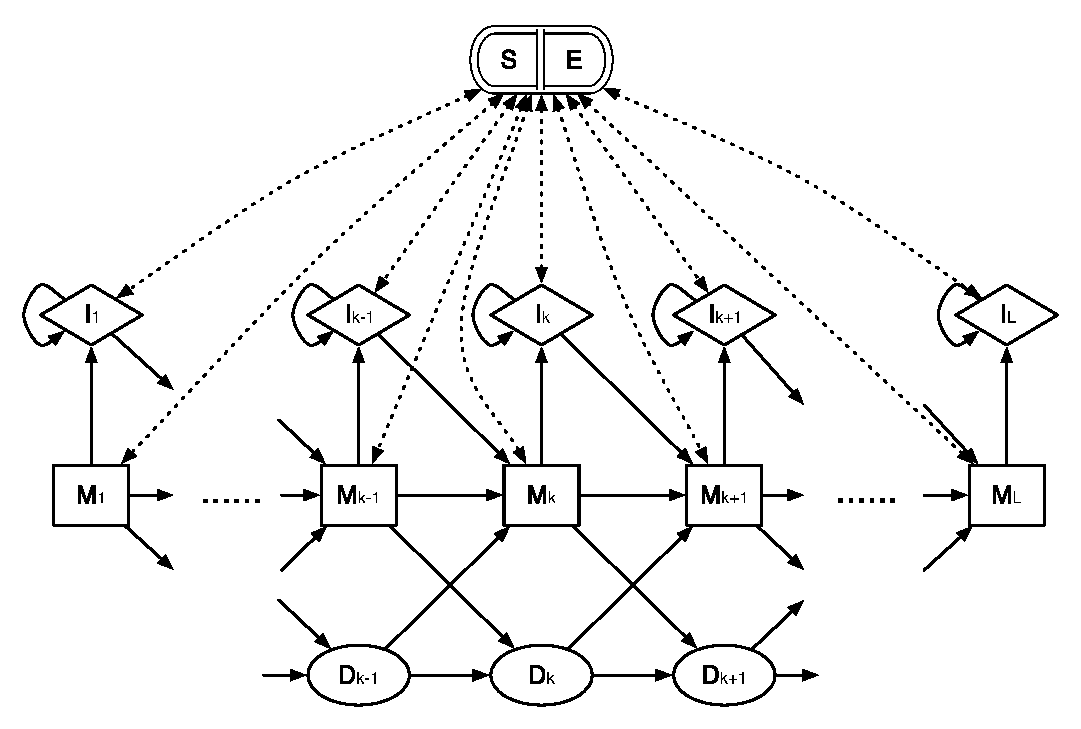
\includegraphics[width=\textwidth]{ahmm}
\caption{A profile HMM for generating sequence reads from a reference
  sequence, where $L$ is the length of the reference sequence, $M$
  states stand for alignment matches, $I$ for alignment insertions to
  the reference and $D$ states for deletions.}\label{fig:ahmm}
\end{figure}

The topology of the profile HMM is given in Fig~\ref{fig:ahmm}. Let
$(M,I,D,S)=(0,1,2,3)$. The transition matrix between different types of
states is
$$
{\bf A}=(a_{ij})_{4\times4}=\left(\begin{array}{cccc}
(1-2\alpha)(1-s) & \alpha(1-s) & \alpha(1-s) & s\\
(1-\beta)(1-s) & \beta(1-s) & 0 & s \\
1-\beta & 0 & \beta & 0 \\
(1-\alpha)/L & \alpha/L & 0 & 0 \\
\end{array}\right)
$$
where $\alpha$ is the gap open probability, $\beta$ is the gap extension
probability and $s=1/(2l)$ with $l$ being the average length of a
read. As to emission probabilities, $P(c_i|D_k)=1$,
$P({\tt\char94}|S)=P({\tt\char36}|S)=1$, $P(c_i|I_k)=0.25$ and
$$
P(b_i|M_k)=e_{ki}=\left\{\begin{array}{ll}
1-10^{-q_i/10} & \mbox{if $r_k=b_i$} \\
10^{-q_i/10}/3 & \mbox{otherwise}
\end{array}\right.
$$
The forward-backward algorithm\footnote{We may adopt a banded
  forward-backward approximation to reduce the time complexity. We may
  also normalize $f_{\tilde{k}}(i)$ for each $i$ to avoid floating point
  underflow.} is as follows:
\begin{eqnarray*}
f_S(0)&=&1\\
f_{M_k}(1)&=&e_{k1}\cdot a_{30}\\
f_{I_k}(1)&=&0.25\cdot a_{31}\\
f_{M_k}(i)&=&e_{ki}\cdot\Big[a_{00}f_{M_{k-1}}(i-1)+a_{10}f_{I_{k-1}}(i-1)+a_{20}f_{D_{k-1}}(i-1)\Big]\\
f_{I_k}(i)&=&0.25\cdot\Big[a_{01}f_{M_k}(i-1)+a_{11}f_{I_k}(i-1)\Big]\\
f_{D_k}(i)&=&a_{02}f_{M_{k-1}}(i)+a_{22}f_{D_{k-1}}(i)\\
f_S(l+1)&=&\sum_{k=1}^La_{03}f_{M_k}(l)+a_{13}f_{I_k}(l)
\end{eqnarray*}
\begin{eqnarray*}
b_S(l+1)&=&1\\
b_{M_k}(l)&=&a_{03}\\
b_{I_k}(l)&=&a_{13}\\
b_{M_k}(i)&=&e_{k+1,i+1}a_{00}b_{M_{k+1}}(i+1)+a_{01}b_{I_k}(i+1)/4+a_{02}b_{D_{k+1}}(i)\\
b_{I_k}(i)&=&e_{k+1,i+1}a_{10}b_{M_{k+1}}(i+1)+a_{11}b_{I_k}(i+1)/4\\
b_{D_k}(i)&=&(1-\delta_{i1})\cdot\Big[e_{k+1,i+1}a_{20}b_{M_{k+1}}(i+1)+a_{22}b_{D_{k+1}}(i)\Big]\\
b_S(0)&=&\sum_{k=1}^Le_{k1}a_{30}b_{M_k}(1)+a_{31}b_{I_k}(1)/4
\end{eqnarray*}
and the likelihood of data is $P(y)=f_S(L+1)=b_S(0)$\footnote{Evaluating
  if $f_S(L+1)=b_S(0)$ helps to check the correctness of the formulae
  and the implementation.}. The posterior probability of a read base
$c_i$ being matching state $\tilde{k}$ (M- or I-typed) is
$f_{\tilde{k}}(i)b_{\tilde{k}}(i)/P(y)$.


\chapter{Modeling Sequencing Errors}

\section{The revised MAQ model}
\subsection{General formulae}
Firstly it is easy to prove that for any $0\le\beta_{nk}<1$ ($0\le k\le n$),
$$
\sum_{k=0}^n(1-\beta_{nk})\prod_{l=0}^{k-1}\beta_{nl}=1-\prod_{k=0}^n\beta_{nk}
$$
where we regard that $\prod_{i=0}^{-1}\beta_{ni}=1$. In particular, when
$\exists k\in[0,n]$ satisfies $\beta_{nk}=0$, we have:
\[\sum^n_{k=0}(1-\beta_{nk})\prod_{i=0}^{k-1}\beta_{ni}=1\]
If we further define:
\begin{equation}\label{equ:alpha-nk}
  \alpha_{nk}=(1-\beta_{nk})\prod_{i=0}^{k-1}\beta_{ni}
\end{equation}
on the condition that some $\beta_{nk}=0$, we have:
\[\sum_{k=0}^n\alpha_{nk}=1\]
\begin{equation*}
\beta_{nk}=1-\frac{\alpha_{nk}}{1-\sum_{i=0}^{k-1}\alpha_{ni}}
=\frac{1-\sum_{i=0}^k\alpha_{ni}}{1-\sum_{i=0}^{k-1}\alpha_{ni}}
=\frac{\sum_{i=k+1}^n\alpha_{ni}}{\sum_{i=k}^n\alpha_{ni}}
\end{equation*}
In the context of error modeling, if we define:
\[
\beta_{nk}\triangleq\left\{\begin{array}{ll}
    \Pr\{\mbox{at least $k+1$ errors}|\mbox{at least $k$ errors out of $n$ bases}\} & (k>0) \\
    \Pr\{\mbox{at least $1$ error out of $n$ bases}\} & (k=0)
  \end{array}\right.
\]
we have $\beta_{nn}=0$, and
$$
\gamma_{nk}\triangleq\prod_{l=0}^{k-1}\beta_{nl}=\Pr\{\mbox{at least $k$ errors out of $n$ bases}\}
$$
then
$$
\alpha_{nk}=(1-\beta_{nk})\gamma_{nk}=\Pr\{\mbox{exactly $k$ errors in $n$ bases}\}
$$

\subsection{Modeling sequencing errors}
Given a uniform error rate $\epsilon$ and independent errors, let
$$
\bar{\alpha}_{nk}(\epsilon)=\binom{n}{k}\epsilon^k(1-\epsilon)^{n-k}
$$
and
$$
\bar{\beta}_{nk}(\epsilon)=\frac{\sum_{i=k+1}^n\bar{\alpha}_{ni}(\epsilon)}{\sum_{i=k}^n\bar{\alpha}_{ni}(\epsilon)}
$$
we can calculate that the probability of seeing at least $k$ errors is
$$
\bar{\gamma}_{nk}(\epsilon)=\prod_{l=0}^{k-1}\bar{\beta}_{nk}(\epsilon)
$$
When errors are dependent, the true $\beta_{nk}$ will be larger than
$\bar{\beta}_{nk}$. A possible choice of modeling this is to let
$$
\beta_{nk}=\bar{\beta}_{nk}^{f_k}
$$
where $0<f_k\le1$ models the dependency for $k$-th error. The
probability of seeing at least $k$ errors is thus
$$
\gamma_{nk}(\epsilon)=\prod_{l=0}^{k-1}\bar{\beta}^{f_l}_{nl}(\epsilon)
$$
For non-uniform errors $\epsilon_1\le\epsilon_2\le\cdots\le\epsilon_n$,
we may approximate $\gamma_{nk}(\vec{\epsilon})$ as
$$
\gamma_{nk}(\vec{\epsilon})=\prod_{l=0}^{k-1}\bar{\beta}^{f_l}_{nl}(\epsilon_{l+1})
$$

\subsection{Practical calculation}
We consider diploid samples only. Let $g\in\{0,1,2\}$ be the number of
reference alleles. Suppose there are $k$ reference alleles whose base
error rates are $\epsilon_1\le\cdots\le\epsilon_k$, and there are $n-k$
alternate alleles whose base error rates are
$\epsilon'_1\le\cdots\le\epsilon'_{n-k}$. We calculate
$$
P(D|0)=\gamma_{nk}(\vec\epsilon)=\prod_{l=0}^{k-1}\bar\beta_{nl}^{f_l}(\epsilon_{l+1})
$$
$$
P(D|2)=\gamma_{nk}(\vec\epsilon')=\prod_{l=0}^{n-k-1}\bar\beta_{nl}^{f_l}(\epsilon'_{l+1})
$$
and
$$
P(D|1)=\frac{1}{2^n}\binom{n}{k}
$$
where $f_l=0.97\eta^{\kappa_l-1}+0.03$ with $\kappa_l$ being the rank of base $l$
among the same type of bases on the same strand, ordered by error
rate. For sequencing data, error rates are usually discretized. We may
precompute $\bar\beta_{nk}(\epsilon)$ for sufficiently large
$n$\footnote{SAMtools precomputes a table for $n\le255$. Given higher
  coverage, it randomly samples $255$ reads.} and all possible
discretized $\epsilon$. Calculating the likelihood of the data is
trivial.

\subsection{The original MAQ model}
The original MAQ models the likelihood of data by
$$
\alpha_{nk}(\epsilon)=(1-\bar\beta^{f_k}_{nk})\prod_{i=0}^{k-1}\bar\beta^{f_i}_{ni}
$$
instead of $\gamma_{nk}(\epsilon)$. For non-uniform errors,
$$
\alpha_{nk}(\vec{\epsilon})=c_{nk}(\bar\epsilon)\cdot\prod_{i=0}^{k-1}\epsilon_{i+1}^{f_i}
$$
where
$$
\log{\bar\epsilon}=\frac{\sum_{i=0}^{k-1}f_i\log\epsilon_{i+1}}{\sum_{i=0}^{k-1}f_i}
$$
and
$$
c_{nk}(\bar\epsilon)\triangleq
\Big[1-\bar\beta^{f_k}_{nk}(\bar\epsilon)\Big]
\prod_{i=0}^{k-1}\Bigg[\frac{\bar\beta_{ni}(\bar\epsilon)}{\bar\epsilon}\Bigg]^{f_i}
$$

The major problem with the original MAQ model is that for $\epsilon$
close to 0.5 and large $n$, the chance of seeing no errors may be so
small that it is even smaller than the chance of seeing all errors
(i.e. $\alpha_{n0}<\alpha_{nn}$). In this case, the model prefers seeing
all errors, which is counterintuitive. The revised model uses the
accumulative probability $\gamma_{nk}$ and does not have this problem.
For small $\epsilon$ and $n$, the original and the revised MAQ models
seem to have similar performance.

\chapter{Modeling Multiple Individuals}

\section{Notations}
Suppose there are $N$ sites from $n$ individuals with $i$-th individual
having $m_i$ ploids. Let $M=\sum_im_i$ be the total number of
chromosomes. Let ${\bf D}=(\vec{D}_1,\ldots,\vec{D}_N)^{\rm T}$ be the
data matrix with vector ${\vec D}_a=(D_{a1},\ldots,D_{an})$ representing
the alignment data for each individual at site $a$. Similary, let
\mbox{${\bf G}=(\vec{G}_a,\ldots,\vec{G}_N)^{\rm T}$} and
\mbox{$\vec{G}_a=(G_{a1},\dots,G_{an})$} be the true genotypes, where
$0\le G_{ai}\le m_i$ equals the number of reference alleles~\footnote{If we
  take the ancestral sequence as the reference, the non-reference allele
  will be the derived allele.}. Define
\begin{equation}
X_a=X_a(\vec{G}_a)\triangleq\sum_iG_{ai}
\end{equation}
to be the number of reference alleles at site $a$ and ${\bf
  X}=(X_1,\ldots,X_N)^{\rm T}$. Also define
$\Phi=(\phi_0,\ldots,\phi_M)$ as the allele frequency spectrum (AFS)
with $\sum_k\phi_k=1$.

For convenience, we may drop the position subscript $a$ when it is
unambiguous in the context that we are looking at one locus.  Also
define
\begin{equation}
P(D_i|g_i)\triangleq\Pr\{D_i|G_i=g_i\}
\end{equation}
to be the likelihood of the data for individual $i$ when the underlying
genotype is known. $P(D_i|g_i)$ is calculated in
Section~\ref{sec:pdg}. And define
\begin{equation}
P(g_i|\phi)\triangleq\binom{m_i}{g_i}\phi^{g_i}(1-\phi)^{m_i-g_i}
\end{equation}
to be the probability of a genotype under the Hardy-Weinberg equilibrium
(HWE), when the site allele frequency is $\phi$.

\section{Estimating AFS}\label{sec:afs}
\subsection{The EM procedure}
We aim to find $\Phi$ that maximizes $P({\bf D}|\Phi)$ by EM. Suppose at
the $t$-th iteration the estimate is $\Phi_t$. We have
$$
\log \Pr\{{\bf D},{\bf X}={\bf x}|\Phi\}=\log \Pr\{{\bf D}|{\bf X}={\bf
  x}\}\Pr\{{\bf X}={\bf x}|\Phi\}=C+\sum_a\log \phi_{x_a}
$$
where $C$ is not a function of $\{\phi_k\}$. The EM $Q$ function
is\footnote{We assume site independency in the following.}
\begin{eqnarray*}
  Q(\Phi|\Phi_t)&=&\sum_{\bf x}\Pr\{{\bf X}={\bf x}|{\bf D},\Phi_t\}\log \Pr\{{\bf D},{\bf X}={\bf x}|\Phi\}\\
  &=&C+\sum_{\bf x}\prod_a \Pr\{X_a=x_a|\vec{D}_a,\Phi_t\}\sum_b\log \phi_{x_b}\\
  &=&C+\sum_{a=1}^N\sum_{x_a=0}^M \Pr\{X_a=x_a|\vec{D}_a,\Phi_t\}\log \phi_{x_a}
\end{eqnarray*}
Requiring $\partial_{\phi_k}(Q-\lambda\sum_l{\phi_l})=0$ leads to
$$
\frac{1}{\phi_k}\sum_a\Pr\{X_a=k|\vec{D}_a,\Phi_t\}-\lambda=0
$$
from which $\lambda$ can be calculated as:
$$
\lambda=\sum_k\sum_a \Pr\{X_a=k|\vec{D}_a,\Phi_t\}=N
$$
and thus at the $(t+1)$ iteration:
\begin{equation}\label{equ:em}
  \phi_k^{(t+1)}=\frac{1}{N}\sum_a\Pr\{X_a=k|\vec{D}_a,\Phi_t\}
\end{equation}
where $\Pr\{X_a=k|\vec{D}_a,\Phi_t\}$ is calculated as follows.

\subsection{The distribution of site reference allele count}
Firstly, as we are only looking at a site from now on, we drop subscript
$a$ for convenience. Without proof\footnote{Supposedly, this can be
  proved by polynomial expansion. Wiki gives a simplified version of
  this formula as
  \href{http://en.wikipedia.org/wiki/Vandermonde's_identity\#Generalized_Vandermonde.27s_identity}{generalized
    Vandermonde's identity}.}, we note that
$$
\binom{M}{k}\equiv\sum_{\vec{g}}\delta_{k,s_n(\vec{g})}\prod_i\binom{m_i}{g_i}
$$
where
$$
s_j(\vec{g})\triangleq\sum_{i=1}^jg_i
$$
and $\delta_{kl}=1$ if $k=l$ and 0 otherwise. The probability of
sampling $\vec{g}$ conditional on $\sum_ig_i=k$ is
$\delta_{k,s_n(\vec{g})}\prod_i\binom{m_i}{g_i}\big/\binom{M}{k}$. With this
preparation, we can calculate\footnote{The derivation below does
  \emph{not} assume Hardy-Weinberg equilibrium.}
\begin{eqnarray*}
\Pr\{\vec{D}|X=k\}&=&\sum_{\vec{g}}\Pr\{\vec{D},\vec{G}=\vec{g}|X=k\}\\
&=&\sum_{\vec{g}}\delta_{k,s_n(\vec{g})}\Pr\{\vec{D}|\vec{G}=\vec{g}\}\Pr\{\vec{G}=\vec{g}|X=k\}\\
&=&\sum_{\vec{g}}\delta_{k,s_n(\vec{g})}\prod_iP(D_i|g_i)\cdot\frac{\prod_j\binom{m_j}{g_j}}{\binom{M}{k}}\\
&=&\frac{1}{\binom{M}{k}}\sum_{\vec{g}}\delta_{k,s_n(\vec{g})}\prod_i\binom{m_i}{g_i}P(D_i|g_i)
\end{eqnarray*}
where $P(D_i|g_i)\triangleq\Pr\{D_i|G_i=g_i\}$ is the likelihood of data
when the underlying genotype is known. To calculate
$\Pr\{\vec{D}|X=k\}$, we define
$$
z_{jk}\triangleq\sum_{g_1=0}^{m_1}\cdots\sum_{g_j=0}^{m_j}\prod_{i=1}^j\binom{m_i}{g_i}P(D_i|g_i)
$$
for $0\le k\le\sum_{i=1}^jm_i$ and 0 otherwise. It can be calculated
iteratively with\footnote{To make it explicit, for diploid samples, if
  $A$ is the reference allele:
$$
z_{jk}=z_{j-1,k}P(D_j|\langle aa\rangle)+2z_{j-1,k-1}P(D_j|\langle Aa\rangle)+z_{j-1,k-2}P(D_j|\langle AA\rangle)
$$
}
\begin{equation}\label{equ:zcal}
z_{jk}=\sum_{g_j=0}^{m_j}z_{j-1,k-g_j}\cdot\binom{m_j}{g_j}P(D_j|g_j)
\end{equation}
with $z_{00}=1$. Thus
$$
\Pr\{\vec{D}|X=k\}=\frac{z_{nk}}{\binom{M}{k}}
$$
and
\begin{equation}\label{equ:postk}
\Pr\{X=k|\vec{D},\Phi\}=\frac{\phi_k\Pr\{\vec{D}|X=k\}}{\sum_l\phi_l\Pr\{\vec{D}|X=l\}}
=\frac{\phi_kz_{nk}/\binom{M}{k}}{\sum_l\phi_lz_{nl}/\binom{M}{l}}
\end{equation}

\subsection{Numerical stability}\label{sec:numsta}
Numerical computation of Eq.~(\ref{equ:zcal}) may lead to floating point
underflow for large $n$. To avoid this, let
$y_{jk}=z_{jk}/\binom{M_j}{k}$, where
$M_j=\sum_{i=1}^jm_i$. Eq.~(\ref{equ:zcal}) becomes
$$
y_{jk}=\left(\prod_{l=0}^{m_j-1}\frac{k-l}{M_{j}-l}\right)\cdot\sum_{g_j=0}^{m_j}\left(\prod_{l=g_j}^{m_j-1}\frac{M_{j-1}-k+l+1}{k-l}\right)\cdot y_{j-1,k-g_j}\cdot\binom{m_j}{g_j}P(D_j|g_j)
$$
In case of diploid samples:
\begin{eqnarray*}
y_{jk}&=&\frac{1}{2j(2j-1)}\Big[(2j-k)(2j-k-1)\cdot y_{j-1,k}P(D_j|\langle aa\rangle)+2k(2j-k)\cdot y_{j-1,k-1}P(D_j|\langle Aa\rangle)\\
&&+k(k-1)\cdot y_{j-1,k-2}P(D_j|\langle AA\rangle)\Big]
\end{eqnarray*}
For haploid samples,
\[
y_{jk}=\frac{1}{M_{j}}\Big[(M_{j-1}-k+1)\cdot y_{j-1,k}P(D_j|a)+k\cdot y_{j-1,k-1}P(D_j|A)\Big]
\]
However, this is not good enough. $y_{jk}$ still decreases exponentially
with increasing $j$. To solve this issue, we rescale $y_{jk}$ for each
$j$. Define
$$
\tilde{y}_{jk}=\frac{y_{jk}}{\prod_{i=1}^j t_i}
$$
where $t_j$ is chosen such that $\sum_l\tilde{y}_{jl}=1$. The posterior is
$$
\Pr\{X=k|\vec{D},\Phi\}=\frac{\phi_k\tilde{y}_{nk}}{\sum_l\phi_l\tilde{y}_{nl}}
$$
It should be noted that $P(D_i|g_i)$ can also be rescaled without
affecting the calculation of the posterior. Furthermore, in the
$\{\tilde{y}_{jk}\}$ matrix, most of cells should be close to
zero. Computation of $\tilde{y}_{nk}$ can be carried in a band instead
of in a triangle. For large $n$, this may considerably reduce computing
time.

\subsection{The initial AFS}
The EM procedure garantees that $\Pr\{{\bf D}|\Phi\}$ monotomically
increases with each iteration and converges to a local optima. However,
if we start this iteration from a bad initial AFS, we may need many
iterations; the iteration is also more likely to be trapped by a local
optima. Here we give several AFS on different conditions under the
infinite-site Wright-Fisher model.

Let $\phi'_k$ be the probability of seeing k non-reference alleles out
of $M$ chromosomes. The frequency of reference alleles $\phi_k$ equals
$\phi'_{M-k}$.

If we take the ancestral sequence as the reference, the standard model
gives $\phi'_k=\theta/k$ and $\phi'_0=1-\sum_k\phi'_k$. When we do not
know if the reference allele is ancestral, the same conclusion still
stands. To see this, for $k>0$:
$$
\phi'_k=\frac{M+1-k}{M+1}\left(\frac{\theta}{k}+\frac{\theta}{M+1-k}\right)=\frac{\theta}{k}
$$
and for $k=0$:
$$
\phi'_k=1-\sum_{k=1}^{M+1}\frac{\theta}{k}+\frac{\theta}{M+1}=1-\sum_{k=1}^{M}\frac{\theta}{k}
$$
where the first term corresponds to the case wherein the reference is
ancestral and the second to the case wherein the reference is derived.

Another useful AFS is the derived allele frequency spectrum on the
condition of loci being discovered from two chromosomes. Under the
Wright-Fisher model, it is:
$$
\phi'_k=\frac{2(M+1-k)}{(M+1)(M+2)}
$$

A third AFS is the derived allele frequency spectrum on the condition of
knowing one derived allele from a chromosome. It is a flat distribution
$$
\phi'_k=\frac{1}{M+1}
$$

\subsection{Joint distribution of allele counts for 2 groups of samples}
Suppose at a locus we have two data sets $\vec{D}'$ and $\vec{D}''$,
with $n'$ samples $m'$ haplotypes and $n''$ samples and $m''$
haplotypes, respectively. Let $n=n'+n''$ and $m=m'+m''$ and
$\vec{D}=\vec{D}'\oplus\vec{D}''$ be the joint of the two data sets. In
addition, let $X'=\sum_{i'}G'_{i'}$, $X''=\sum_{i''}G''_{i''}$ and
$X=X'+X''$. We have
$$
\Pr\{\vec{D}'|X'=k'\}=\frac{z'_{n'k'}}{\binom{M'}{k'}}
$$
$$
\Pr\{\vec{D}''|X''=k''\}=\frac{z''_{n''k''}}{\binom{M''}{k''}}
$$
and
$$
\Pr\{\vec{D}',\vec{D}''|X'=k',X''=k''\}=\Pr\{\vec{D}'|X'=k'\}\Pr\{\vec{D}''|X''=k''\}=\frac{z'_{n'k'}z''_{n''k''}}{\binom{M'}{k'}\binom{M''}{k''}}
$$
where
$$
z'_{j'k'}\triangleq\sum_{g'_1=0}^{m'_1}\cdots\sum_{g'_j=0}^{m'_j}\prod_{i'=1}^{j'}\binom{m'_i}{g'_i}P(D'_i|g'_i)
$$
and similar to $z''_{j''k''}$. If we note that
$$
\Pr\{X'=k',X''=k''|\Phi\}=\phi_k\cdot\frac{\binom{M'}{k'}\binom{M''}{k''}}{\binom{M}{k}}
$$
and by definition
$$
z_{nk}=z_{n'+n'',k'+k''}=\sum_{\{k',k''|k'+k''=k\}}z'_{n'k'}z''_{n''k''}
$$
we have
$$
\Pr\{\vec{D}|\Phi\}=\sum_k\Pr\{\vec{D},X=k|\Phi\}=\sum_{k',k''}\Pr\{\vec{D}',\vec{D}'',X'=k',X''=k''|\Phi\}
$$
Thus we can derive the joint distribution:
\begin{equation}
\Pr\{X'=k',X''=k''|\vec{D},\Phi\}=\frac{\phi_{k'+k''}z'_{n'k'}z''_{n''k''}\big/\binom{M}{k'+k''}}{\sum_l\phi_lz_{nl}\big/\binom{M}{l}}
\end{equation}
If we let $y_{jk}=z_{jk}/\binom{M_j}{k}$ as in Section~\ref{sec:numsta},
$$
\Pr\{X'=k',X''=k''|\vec{D},\Phi\}=\frac{\phi_{k'+k''}y'_{n'k'}y''_{n''k''}}{\sum_l\phi_ly_{nl}}\cdot\frac{\binom{M'}{k'}\binom{M''}{k''}}{\binom{M'+M''}{k'+k''}}
$$
This derivation can be extended to arbitrary number of data sets.

To test the association between the two groups of samples, we may use
the following statistics:
\[
P=\sum_{k',k''}\Pr\{X'=k',X''=k''|\vec{D},\Phi\}\cdot P(\chi^2(k',n'-k',k'',n''-k'')|1)
\]
where $\chi^2(n_{11},n_{12},n_{21},n_{22})$ gives the $\chi^2$ statistics of
a 2-by-2 contingency table and $P(\chi^2|1)$ computes the $P$-value of an 1-degree
$\chi^2$ statistics. Theoretically speaking, the equation above is not correct.
As a result, the $P$-value computed this way tends to underestimate the significance
on real data. Nonetheless, the relative value is still useful and this statistics
has a nice feature that when the data has little ambiguity, it approaches
the standard 1-degree $\chi^2$ used in GWAS.



\section{EM estimate of site statistics}

\subsection{Estimating site allele frequency assuming HWE}
Here we aim to find $\phi$ that maximises $\Pr\{\vec{D}|\phi\}$. We have:
$$\log \Pr\{\vec{D},\vec{G}=\vec{g}|\phi\}=\log\prod_iP(D_i|g_i)P(g_i|\phi)=C+\sum_i\log P(g_i|\phi)$$
Given an estimate $\phi_t$ at the $t$-th iteration, the $Q(\phi|\phi_t)$
function of EM is:
\begin{eqnarray*}
  Q(\phi|\phi_t)&=&\sum_{\vec{g}}\Pr\{\vec{G}=\vec{g}|\vec{D},\phi_t\}\log \Pr\{\vec{D},\vec{G}=\vec{g}|\phi\}\\
  &=&C+\sum_{\vec{g_i}}\prod_i\Pr\{G_i=g_i|D_i,\phi_t\}\sum_j\log P(g_j|\phi)\\
  &=&C+\sum_{i=1}^n\sum_{g_i=0}^{m_i}\Pr\{G_i=g_i|D_i,\phi_t\}\log P(g_i|\phi)\\
  &=&C+\sum_i\sum_{g_i}\Pr\{G_i=g_i|D_i,\phi_t\}\log_i \binom{m_i}{g_i}\phi^{g_i}(1-\phi)^{m_i-g_i}\\
  &=&C'+\sum_i\sum_{g_i}\Pr\{G_i=g_i|D_i,\phi_t\}\Big[g_i\log\phi+(m_i-g_i)\log(1-\phi)\Big]\\
\end{eqnarray*}
Requiring $\partial_{\phi}Q\Big|_{\phi=\phi_{t+1}}=0$ gives:
$$\frac{1}{\phi_{t+1}(1-\phi_{t+1})}\sum_i\sum_{g_i}\Pr\{G_i=g_i|D_i,\phi_t\}(g_i-m_i\phi_{t+1})=0$$
Thus
\begin{equation}\label{equ:freq1}
\phi_{t+1}=\frac{1}{\sum_jm_j}\sum_i\sum_{g_i}g_i\Pr\{G_i=g_i|D_i,\phi_t\}
=\frac{1}{M}\sum_i\frac{\sum_{g_i}g_iP(D_i|g_i)P(g_i|\phi_t)}{\sum_{g_i}P(D_i|g_i)P(g_i|\phi_t)}
\end{equation}
which is the EM estimate at the $(t+1)$-th iteration and also the
expected reference allele frequency.

\subsection{Estimating genotype frequency}
In the previous section, we estimate the site allele frequency assuming Hardy-Weinberg equilibrium (HWE).
We can actually relax this assumption when all samples have the sample diploidy.
Let $m=m_1=\cdots=m_n$ and $\vec{\phi}=\{\phi_0,\phi_1,\ldots,\phi_m\}$ be the vector of
genotype frequency satisfying $\sum_g\phi_g=1$. It is easy to compute the $Q$-function:
$$
Q(\vec{\phi}|\vec{\phi}^{(t)})=C+\sum_{i=1}^n\sum_{g=0}^m\Pr\{G_i=g|D_i,\vec{\phi}^{(t)}\}\log\phi_g
$$
Requiring $\partial_{\phi_g}\big[Q(\vec{\phi}|\vec{\phi}^{(t)})-\lambda\sum_{g'}\phi_{g'}\big]\Big|_{\phi_g=\phi_g^{(t+1)}}$=0 gives $\lambda=n$
and thus
$$
\phi_g^{(t+1)}=\frac{1}{n}\sum_{i=1}^n\Pr\{G_i=g|D_i,\vec{\phi}^{(t)}\}=\frac{1}{n}\sum_{i=1}^n\frac{P(D_i|g)\phi_g^{(t)}}{\sum_{g'}P(D_i|g')\phi_{g'}^{(t)}}
$$
Obviously, $\sum_g\phi_g^{(t+1)}=1$ as it should be. This estimate is useful to test HWE.

\subsection{Estimating two-locus LD}
In this section, we only consider diploid samples
(i.e. $m_1=\cdots=m_n=2$). Let ${\bf D}=(\vec{D},\vec{D}')$ be the data
at two loci, respectively; and $H_i$ and $H^{\dag}_i$ be the two
underlying haplotypes for individual $i$ with $H_i\in\{0,1,2,3\}$
representing one of the four possible haplotypes at the 2 loci. We write
${\bf H}=\overrightarrow{(H_i,H^{\dag}_i)}$ as a haplotype configuration of the
samples. Define
$$
\mathcal{G}_{hk}=\mathcal{G}_{kh}=\lfloor h/2\rfloor+\lfloor k/2\rfloor
$$
$$
\mathcal{G}'_{hk}=\mathcal{G}'_{kh}=(h\mod 2)+(k\mod 2)
$$
which calculate the genotype of each locus, respectively.
\begin{eqnarray*}
  Q(\vec{\phi}|\vec{\phi}^{(t)})&=&\sum_{\bf h}P({\bf H}={\bf h}|{\bf D},\vec{\phi}^{(t)})\log\Pr\{{\bf D},{\bf H}={\bf h}|\vec{\phi}\}\\
  &=&C+\sum_{\bf h}\prod_i\Pr\{H_i=h_i,H^{\dag}_i=h^{\dag}_i|{\bf D},\vec{\phi}^{(t)}\}\sum_j\log P(h_j,h^{\dag}_j|\vec{\phi})\\
  &=&C+\sum_i\sum_{h_i}\sum_{h^{\dag}_i}\Pr\{H_i=h_i,H^{\dag}_i=h^{\dag}_i|{\bf D},\vec{\phi}^{(t)}\}\sum_j\log(\phi_{h_i}\phi_{h^{\dag}_i})
\end{eqnarray*}
%P(\mathcal{G}(h_i,h^{\dag}_i)|\vec{D},\vec{\phi})P(\mathcal{G}'(h_i,h^{\dag}_i)|\vec{D}',\vec{\phi})\log(\phi_{h_i}\phi_{h^{\dag}_i})
Solving $\partial_{\phi_k}Q-\lambda=0$ gives
\begin{eqnarray*}
\phi_k&=&\frac{1}{2n}\sum_i\sum_h\left(\Pr\{H_i=h,H^{\dag}_i=k|{\bf D},\vec{\phi}^{(t)}\}+\Pr\{H_i=k,H^{\dag}_i=h|{\bf D},\vec{\phi}^{(t)}\}\right)\\
&=&\frac{\phi^{(t)}_k}{2n}\sum_{i=1}^n\frac{\sum_{h}\phi^{(t)}_h\big[P(D_i|{\cal G}_{hk})P(D'_i|{\cal G}'_{hk})+P(D_i|{\cal G}_{kh})P(D'_i|{\cal G}'_{kh})\big]}{\sum_{k',h}\phi^{(t)}_{k'}\phi^{(t)}_hP(D_i|{\cal G}_{hk'})P(D'_i|{\cal G}'_{hk'})}\\
&=&\frac{\phi^{(t)}_k}{n}\sum_{i=1}^n\frac{\sum_{h}\phi^{(t)}_hP(D_i|{\cal G}_{hk})P(D'_i|{\cal G}'_{hk})}{\sum_{k',h}\phi^{(t)}_{k'}\phi^{(t)}_hP(D_i|{\cal G}_{hk'})P(D'_i|{\cal G}'_{hk'})}
\end{eqnarray*}



\section{An alternative model assuming HWE}
In Section~\ref{sec:afs}, $\phi_k$ in $\Phi=\{\phi_k\}$ is interpreted
as the probability of seeing exactly $k$ alleles from $M$
chromosomes. Under this model, the prior of a genotype configuration is
$$
\Pr\{\vec{G}=\vec{g}|\Phi\}=\phi_{s_n(\vec{g})}\frac{\prod_i\binom{m_i}{g_i}}{\binom{M}{s_n(\vec{g})}}
$$
and the posterior is
$$
\Pr\{\vec{G}=\vec{g}|\vec{D},\Phi\}=\frac{\phi_{s_n(\vec{g})}}{\Pr\{\vec{D}|\Phi\}}\cdot\frac{\prod_i\binom{m_i}{g_i}P(D_i|g_i)}{\binom{M}{s_n(\vec{g})}}
$$
Suppose we want to calculate the expectation of $\sum_if_i(g_i)$, we can
$$
\sum_i\sum_{\vec{g}}f_i(g_i)\Pr\{\vec{G}=\vec{g}|\vec{D},\Phi\}
=\frac{1}{\Pr\{\vec{D}|\Phi\}}\sum_i\sum_k\frac{\phi_k}{\binom{M}{k}}\sum_{\vec{g}}\delta_{k,s_n(\vec{g})}f_i(g_i)\prod_j\binom{m_j}{g_j}P(D_j|g_j)
$$
Due to the presence of $\delta_{k,s_n(\vec{g})}$, we are unable to
reduce the formula to a simpler form. Although we can take a similar
strategy in Section~\ref{sec:afs} to calculate $\sum_k\sum_{\vec{g}}$,
which is $O(n^2)$, another sum $\sum_i$ will bring this calculation to
$O(n^3)$. Even calculating the marginal probability
$\Pr\{G_i=g_i|\vec{D},\Phi\}$ requires this time complexity. All the
difficulty comes from that individuals are correlated conditional on
$\{X=k\}$.

An alternative model is to interpret the AFS as the discretized AFS of
the population rather than for the observed individuals. We define the
population AFS discretized on $M$ chromosomes as
$\Phi'=\{\phi'_k\}$. Under this model,
$$
\Pr\{\vec{G}=\vec{g}|\Phi'\}=\sum_k\phi_k\prod_iP(g_i|k/M)
$$
$$
\Pr\{\vec{G}=\vec{g},\vec{D}|\Phi'\}=\sum_k\phi_k\prod_iP(D_i|g_i)P(g_i|k/M)
$$
$$
\Pr\{\vec{D}|\Phi'\}=\sum_{\vec{g}}\Pr\{\vec{G}=\vec{g},\vec{D}|\Phi'\}
=\sum_{k=0}^M\phi'_k\prod_{i=1}^n\sum_{g_i=0}^{m_i}P(D_i|g_i)P(g_i|k/M)
$$
and
\begin{eqnarray}\label{equ:fexp}
&&\sum_i\sum_{\vec{g}}f_i(g_i)\Pr\{\vec{G}=\vec{g}|\vec{D},\Phi'\}\\\nonumber
&=&\frac{1}{\Pr\{\vec{D}|\Phi'\}}\sum_i\sum_{\vec{g}}f_i(g_i)\sum_k\phi'_k\prod_jP(D_j|g_j)P(g_j|k/M)\\\nonumber
&=&\frac{1}{\Pr\{\vec{D}|\Phi'\}}\sum_k\phi'_k\sum_if_i(g_i)P(D_i|g_i)P(g_i|k/M)\prod_{j\not=i}\sum_{g_j}P(D_j|g_j)P(g_j|k/M)\\\nonumber
&=&\frac{1}{\Pr\{\vec{D}|\Phi'\}}\sum_k\phi'_k\left[\prod_i\sum_{g_i}P(D_i|g_i)P(g_i|k/M)\right]\cdot\left[\sum_i\frac{\sum_{g_i}f_i(g_i)P(D_i|g_i)P(g_i|k/M)}{\sum_{g_i}P(D_i|g_i)P(g_i|k/M)}\right]
\end{eqnarray}
The time complexity of this calculation is $O(n^2)$. Consider that if
$f_i(g_i)=g_i$, $X=\sum_if_i(G_i)$. We can easily calculate
$E(X|\vec{D},\Phi')$ with the formula above.

\subsection{Posterior distribution of the allele count}
Under the alternative model, we can also derive the posterior
distribution of $X$, $\Pr\{X=k|\vec{D},\Phi'\}$ as follows.
$$
\Pr\{X=k|\Phi'\}=\binom{M}{k}\sum_{l=0}^M\phi'_l\left(\frac{l}{M}\right)^k\left(1-\frac{l}{M}\right)^{M-k}
$$
Then
\begin{equation}\label{equ:pdk-alt}
\Pr\{\vec{D},X=k|\Phi'\}=z_{nk}\sum_{l=0}^M\phi'_l\left(\frac{l}{M}\right)^k\left(1-\frac{l}{M}\right)^{M-k}
\end{equation}

In fact, we also have an alternative way to derive this
$\Pr\{\vec{D},X=k|\Phi'\}$. Let $\phi'$ be the true site allele
frequency in the population. Assuming HWE, we have
\begin{eqnarray}\label{equ:pdk2}
\Pr\{X=k,\vec{D}|\phi'\}&=&\sum_{\vec{g}}\delta_{k,s_n(\vec{g})}\Pr\{\vec{D}|\vec{G}=\vec{g}\}\Pr\{\vec{G}=\vec{g}|\phi'\}\\\nonumber
&=&\sum_{\vec{g}}\delta_{k,s_n(\vec{g})}\prod_iP(D|g_i)\binom{m_i}{g_i}\phi'^{g_i}(1-\phi')^{m_i-g_i}\\\nonumber
&=&\phi'^k(1-\phi')^{M-k}\sum_{\vec{g}}\delta_{k,s_n(\vec{g})}\prod_i\binom{m_i}{g_i}P(D_i|g_i)\\\nonumber
&=&\phi'^k(1-\phi')^{M-k}z_{nk}
\end{eqnarray}
Summing over the AFS gives
\begin{equation*}
\Pr\{\vec{D},X=k|\Phi'\}=\sum_l\phi'_l\Pr\{X=k,\vec{D}|\phi'=l/M\}
\end{equation*}
which is exactly Eq.~(\ref{equ:pdk-alt}). It is worth noting that
$E(X|\vec{D},\Phi')$ calculated by Eq.~(\ref{equ:pdk2}) is identical to
the one calculated by Eq.~(\ref{equ:fexp}), which has been numerically
confirmed.

In practical calculation, the alternative model has very similar
performance to the method in Section~\ref{sec:afs} in one
iteration. However, in proving EM, we require $\Pr\{X=k|\Phi\}=\phi_k$,
which does not stand any more in the alternative
interpretation. Iterating Eq.~(\ref{equ:pdk-alt}) may not monotonically
increase the likelihood function. Even if this was also another
different EM procedure, we have not proved it yet. Yi {\it et al.}
(2010) essentially calculates Eq.~(\ref{equ:pdk2}) for $\phi'$ estimated
from data without summing over the AFS. Probably this method also
delivers similar results, but it is not theoretically sound and may not
be iterated, either.

\section{Likelihood of data given genotype}\label{sec:pdg}
Given a site covered by $k$ reads from an $m$-ploid individual, the
sequencing data is:
\[
D=(b_1,\dots,b_k)=(\underbrace{1,\ldots,1}_l,\underbrace{0,\ldots,0}_{k-l})
\]
where 1 stands for a reference allele and 0 otherwise. The $j$-th base
is associated with error rate $\epsilon_j$, which is the larger error
rate between sequencing and alignment errors. We have
\begin{equation}
P(D|0)=\prod_{j=1}^l\epsilon_j\prod_{j=l+1}^k(1-\epsilon_j)=\left(1-\sum_{j=l+1}^k\epsilon_j+o(\epsilon^2)\right)\prod_{j=1}^l\epsilon_j
\end{equation}
\begin{equation}
P(D|m)=\left(1-\sum_{j=1}^l\epsilon_j+o(\epsilon^2)\right)\prod_{j=l+1}^k\epsilon_j
\end{equation}
For $0<g<m$:
\begin{eqnarray}\label{eq:gd}
P(D|g)&=&\sum_{a_1=0}^1\cdots\sum_{a_k=0}^1\Pr\{D|B_1=a_1,\ldots,B_k=a_k\}\Pr\{B_1=a_1,\ldots,B_k=a_k|g\}\\\nonumber
&=&\sum_{\vec{a}}\left(\frac{g}{m}\right)^{\sum_j a_j}\left(1-\frac{g}{m}\right)^{k-\sum_j a_j}\cdot\prod_j p_j(a_j)\\\nonumber
&=&\left(1-\frac{g}{m}\right)^k\prod_j\sum_{a=0}^1 p_j(a)\left(\frac{g}{m-g}\right)^a\\\nonumber
&=&\left(1-\frac{g}{m}\right)^k\prod_{j=1}^l\left(\epsilon_j+\frac{g}{m-g}(1-\epsilon_j)\right)\prod_{j=l+1}^k\left(1-\epsilon_j+\frac{\epsilon_jg}{m-g}\right)\\\nonumber
&=&\left(1-\frac{g}{m}\right)^k\left\{\left(\frac{g}{m-g}\right)^l+\left(1-\frac{g}{m-g}\right)\left(\sum_{j=1}^l\epsilon_j-\sum_{j=l+1}^k\epsilon_j\right)+o(\epsilon^2)\right\}
\end{eqnarray}
where $a=\sum_j a_j$ and
$$
p_j(a)=\left\{\begin{array}{ll}
\epsilon_j & \mbox{$a=1$}\\
1-\epsilon_j & \mbox{$a=0$}\\
\end{array}\right.
$$
In the bracket of Eq.~\ref{eq:gd}, the first term explains the deviation between $l/k$ and
$g/m$ by imperfect sampling, while the second term explains the
deviation by sequencing errors. The second term can be ignored when $k$
is small but may play a major role when $k$ is large. In particular, for
$m=2$, $P(D|1)=2^{-k}$, independent of sequencing errors.

In case of dependent errors, we may replace:
\[\epsilon_1<\epsilon_2<\cdots<\epsilon_l\]
with
\[\epsilon'_j=\epsilon_j^{\alpha^{j-1}}\]
where parameter $\alpha\in[0,1]$ addresses the error dependency.

\section{Multi-sample SNP calling and genotyping}

The probability of the site being polymorphic is
$\Pr\{X=0|\vec{D},\Phi\}$. For individual $i$, we may estimate the
genotype $\hat{g}_i$ as:
$$
\hat{g}_i=\argmax_{g_i} \Pr\{G_i=g_i|D_i,\phi_E\}=\argmax_{g_i}\frac{P(D_i|g_i)P(g_i|\phi_E)}
{\sum_{h_i}P(D_i|h_i)P(h_i|\phi_E)}
$$
where
$$
\phi_E=E(X|\vec{D},\Phi)/M
$$
This estimate of genotypes may not necessarily maximize the posterior
probability $P(\vec{g}|\vec{D})$, but it should be good enough in
practice. However, it should be noted that $\sum_i\hat{g}_i$ is usually
a bad estimator of site allele frequency. The max-likelihood estimator
by Eq. \eqref{equ:freq1} is much better.

\end{document}
